\subsubsection{ Digit readers }

\begin{itemize}
% 0 to l - 1 means L
% 0 to l - 2 means L - 1
% 2MSB:  in: L-2,  out=L-1
% MSB;    in: L-1 , out=L
\item For each $i = 1,2,3$,
               $j = 0,\ldots,l-2$,
               $u \in \{0, 1\}^j$, and
               $\inc \in \{{\tt increment}, {\tt copy} \}$:
    \begin{itemize}
        \item if $j = 0$:
        create
        $\begin{aligned}[t]
            \cread(& \left\langle {\tt CounterRead}, i, \lambda, \inc \right\rangle, \\
                   & \left\langle {\tt CounterRead}, i, 0,      \inc \right\rangle, \\
                   & \left\langle {\tt CounterRead}, i, 1,      \inc \right\rangle \;)
        \end{aligned}$\\ from the general gadget in Figure~\ref{fig:counter_read}.

        \item else:
        create $\begin{aligned}[t]
        \cread(& \left\langle {\tt CounterRead}, i, u,  \inc \right\rangle, \\
               & \left\langle {\tt CounterRead}, i, 0u, \inc \right\rangle, \\
               & \left\langle {\tt CounterRead}, i, 1u, \inc \right\rangle \;)
        \end{aligned}$\\ from the general gadget in Figure~\ref{fig:counter_read}.
    \end{itemize}

\end{itemize}

\begin{itemize}

    \item For each $i = 1,2,3$ and each $u \in \{0, 1\}^{l-1}$:

    \begin{itemize}
        \item Create $\begin{aligned}[t]
            \cread(& \left\langle {\tt CounterRead}, i,  u, {\tt copy} \right\rangle,
                     \left\langle {\tt PreWarp},     i, 0u, {\tt copy} \right\rangle,
                     \left\langle {\tt PreWarp},     i, 1u, {\tt copy} \right\rangle \;)
        \end{aligned}$\\from the general gadget in Figure~\ref{fig:counter_read}.
    \end{itemize}


Since the counter must only increment the current value if the result will be less than $m$,
the \\{\cread} gadgets that have both an {\tt increment} signal and input size of $l - 2$ must
first right shift the bits 2 spots, and then for each possible value after reading one more bit,
check whether that value is less than $m - 1$. % counting in base-M implies that each digit must be less than M %.
%
Basically, if the next bit read is a 0, we check if the current value + 1 is less than $m$.
%
%
%
% If the counter is counting in base 8, (m is 8), then each digit has 3 (value) + 2 (indicator) bits.
% The max digit value is "111"
% Here we'd be on the last/most significant bit, so we've read "0100", and now let's pretend the next
% bit is a "1", so the output would be "10100" IF this was a copy row.
%
% But we're incrementing, so focusing only on the digit value of "101"...
%
% Since the next bit is in the log(M) - 1's index, this means we must add 2^ log(M) - 1 to
% "01" (the current value). We call this the final value of the digit.
%
% So adding 2^log2(M) - 1 to the final value, we get "101". Then, once we know the final value,
% we check to see if the final value + 1 is less than M. If it is, the digit can be incremented
% and we change the increment signal to a copy signal and pass along the final value + 1 as the next digit
% to write, otherwise we output all zeroes and keep the increment signal.
%
If the next bit read is a 1, we check if current value + $2^{\log (m) - 1}$ + 1 is less than $m$.
%
For both cases, if the counter can increment the current value, then
the {\cread} gadgets output the incremented value to the {\prewarp} gadgets and output a {\tt copy}
signal. Otherwise, if the counter is unable to increment the value, it outputs signal in which the bits
of the digit is all zeroes and it will propagate the {\tt increment} signal to the next digit.

    \begin{algorithm}
        \caption{Incrementing and halting}\label{asda}
        \begin{algorithmic}[1]
            \Function{ReadMSB}{}
                \If{$u$ ends with ``11"}
                    \State $out0 \gets \left\langle {\tt halt} \right\rangle$.
                    \State $out1 \gets \left\langle {\tt halt} \right\rangle$.
                \Else
                    \State $guess0 \gets 0u >> 2$.
                    \State $guess1 \gets 1u >> 2$.
                    \If{$convertToDecimal(guess0) + 1 < m - 1$}
                        \State $out0 \gets \left\langle {\tt PreWarp}, i, convertToBinary(convertToDecimal(guess0) + 1) + u[1] + [0], {\tt copy} \right\rangle$.
                    \Else
                        \State $out0 \gets \left\langle {\tt PreWarp}, i, repeat(``0", m) + u[1] + u[0], {\tt increment} \right\rangle$.
                    \EndIf
                    \If{$convertToDecimal(guess1) + 1 < m - 1$}
                        \State $out1 \gets \left\langle {\tt PreWarp}, i, convertToBinary(convertToDecimal(guess1) + 1) + u[1] + [0], {\tt copy} \right\rangle$.
                    \Else
                        \State $out1 \gets \left\langle {\tt PreWarp}, i, repeat(``0", m) + u[1] + u[0], {\tt increment} \right\rangle$.
                    \EndIf
                \EndIf
            \EndFunction
        \end{algorithmic}
    \end{algorithm}

    \begin{itemize}
        \item
        Create $\begin{aligned}[t]
                   \cread(& \left\langle {\tt CounterRead}, i, u, {\tt increment} \right\rangle, out0, out1 \;)
               \end{aligned}$\\from the general gadget in Figure~\ref{fig:counter_read}.
    \end{itemize}
\end{itemize}

\begin{figure}[H]
    \centering
    \subcaptionbox{{\tt Counter\_Read\_0} \label{fig:counter_read_0}}
    {\makebox[0.24\textwidth][c]{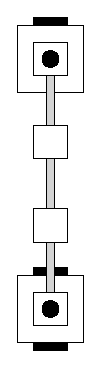
\includegraphics[width=0.33in]{counter_read_0}}}%
    ~
    \subcaptionbox{{\tt Counter\_Read\_1} \label{fig:counter_read_1}}
    {\makebox[0.24\textwidth][c]{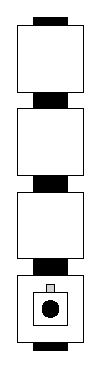
\includegraphics[width=0.33in]{counter_read_1}}}%
    ~
    \subcaptionbox{Digits 1, 2, \& 3 - general overview \label{fig:counter_read_general}}
    {\makebox[0.24\textwidth][c]{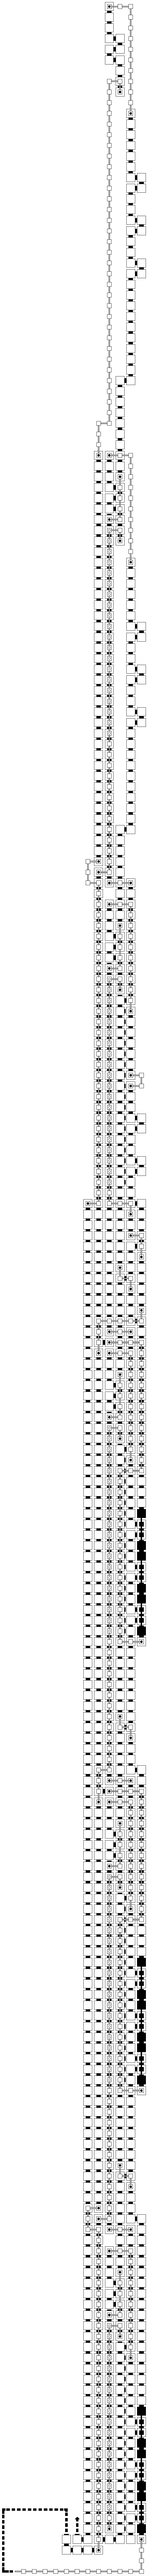
\includegraphics[width=0.45in]{overviews/general/counter_read}}}%
    ~
\end{figure}
\begin{figure}[H]\ContinuedFloat
    \centering
    \subcaptionbox{Digit 1 - case 1 overview  \label{fig:counter_read_case1}}
    {\makebox[0.24\textwidth][c]{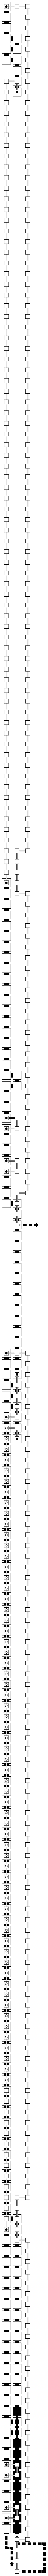
\includegraphics[width=0.45in]{overviews/case1/counter_read_1_op_msr_msd}}}%
    ~
    \subcaptionbox{Digits 1 \& 2 - case 2 overview \label{fig:counter_read_case2}}
    {\makebox[0.24\textwidth][c]{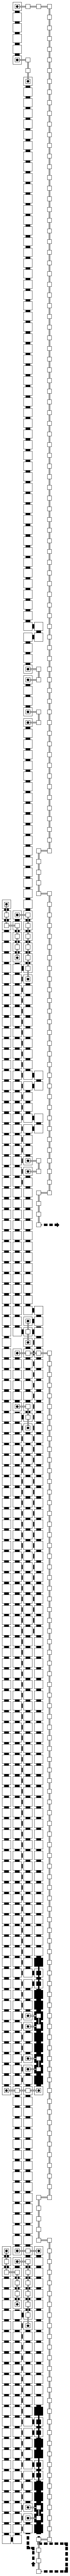
\includegraphics[width=0.45in]{overviews/case2/counter_read}}}%
    ~
    \caption{\label{fig:counter_read} The {\cread} gadgets.}
\end{figure}